\documentclass{beamer}

\usetheme{simple}

\usepackage{lmodern}
\usepackage[scale=2]{ccicons}

\usepackage[utf8]{inputenc}
\usepackage[czech]{babel}
\usepackage{graphicx}
\usepackage[letterspace=100]{microtype}

\title{Jak vylepšit design pomocí typografie}
\subtitle{Tipy a triky}
\date{\today}
\author{Martin Omacht}

\begin{document}

\maketitle

\begin{frame}{Mezery mezi písmeny}    
	\begin{itemize}
		\item Upravením mezer mezi písmeny lze zdůraznit význam textu nebo navodit náladu.
		\item Pozor na zachování čitelnosti
	\end{itemize}
	\begin{center}
		\begin{figure}[h]
			
\includegraphics[width=90mm]{manhattan.jpg}
			\caption{Tučné písmo a zúžené mezery vyzdvyhují pocit velkoměsta na pozadí.}
		\end{figure}
	\end{center} 
\end{frame}





\begin{frame}{Zvolte styl písma odpovídající obsahu}
	\begin{itemize}
		\item Podle cílové audience
		\begin{itemize}
			\item Děti\,--\,hravé písmo
			\item Dospělí\,--\,serziózní písmo
		\end{itemize}
		\item Podle stylu
		\begin{itemize}
			\item Moderní styl\,--\,tenké bezpatkové písmo 
			\item Tradiční\,--\,patkové písmo nebo okrasné písmo (ručně psané)
		\end{itemize}
	\end{itemize}

	\begin{center}
		\begin{figure}[h]
			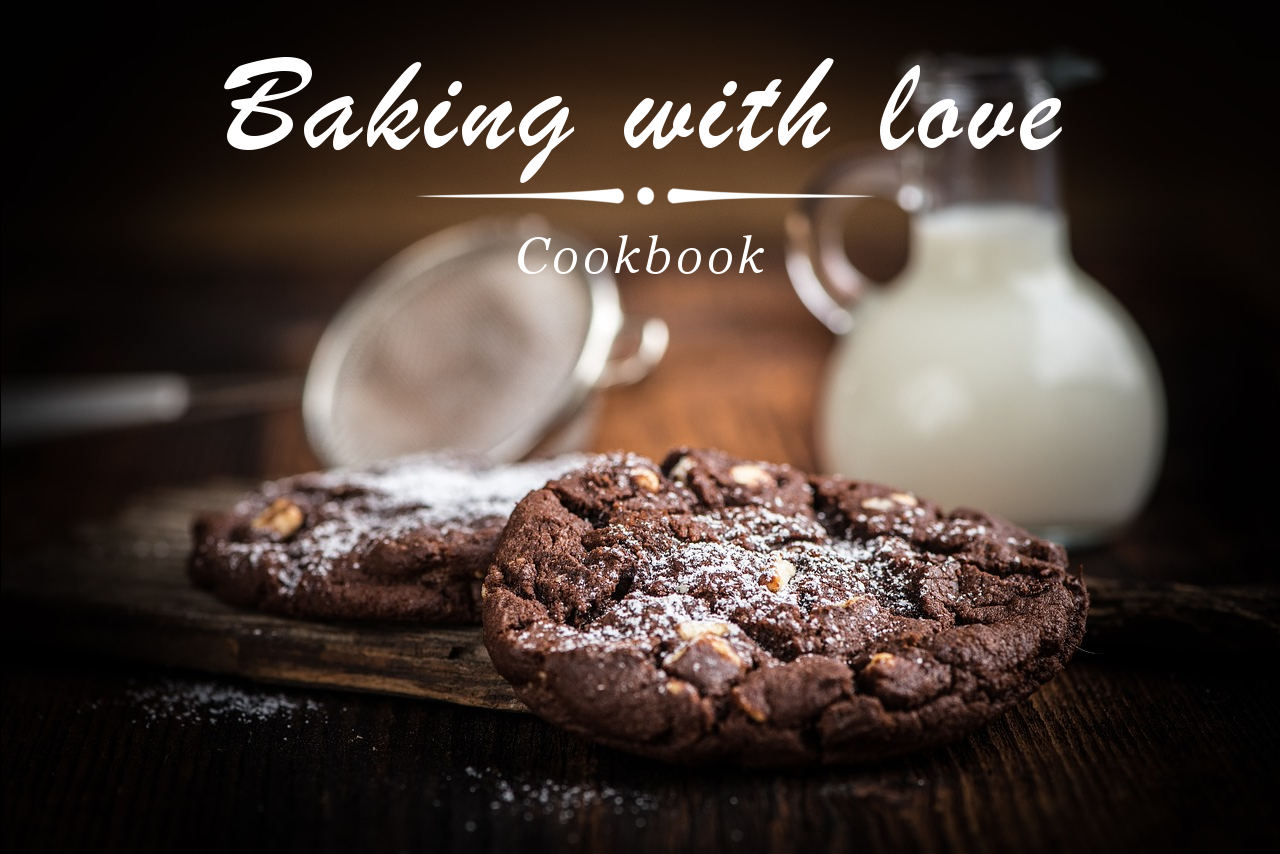
\includegraphics[width=65mm]{cookbook.jpg}
			\caption{Písmo nadpisu navozuje pocit tradiční domácí kuchařky.}
		\end{figure}
	\end{center} 
\end{frame}




\begin{frame}{Hrajte si s okrasnýma znakama}   
	\begin{itemize}
		\item Zkuste použít znaky z okrasných písem jako spojující znaky nebo prvky designu.
	\end{itemize}
	\vfill
	\begin{center}
		\begin{figure}[h]
			
\includegraphics[width=80mm]{tipsandtricks.png}
			\caption{Jako spojení dvou slov zde byl použit okrasný amprsand.}
		\end{figure}
	\end{center} 
\end{frame}




\begin{frame}{Krátké nadpisy velkými písmeny}
	\begin{itemize}
		\item Nevhodné pro delší nadpisy nebo text
		\item \textbf{TUČNÉ NADPISY} upoutají pozornost
		\item {\lsstyle ZVĚTŠENÉ MEZERY} a tenké písmo vypadají moderněji
	\end{itemize}
\end{frame}




\begin{frame}{Kombinujte tučné a tenké písma}
	\begin{itemize}
		\item Použitím různých řezů stejného písma se dájí odlišit slova bez přidání mezery.
	\end{itemize}

	\begin{center}
		\begin{figure}[h]
			
\includegraphics[width=90mm]{acrylicbar.jpg}
			\caption{Slova \uv{acrylic} a \uv{bar} byly odděleny změnou řezu písma.}
		\end{figure}
	\end{center} 
\end{frame}



\begin{frame}
	\begin{center}
		{\huge Děkuji za pozornost}
	\end{center}
\end{frame}

\begin{frame}[t]{Použité zdroje}
	\begin{itemize}
		\item Typography Tutorial: Terms, Tips and Tricks\\
		\small\texttt{https://designschool.canva.com/blog/typography-tutorial/}
	\end{itemize}
\end{frame}

\end{document}